\subsection{Modelo OSI}

El modelo OSI es un modelo que abstrae en 7 capas los protocolos involucrados en la comunicación entre dos nodos en una red.

\begin{center}
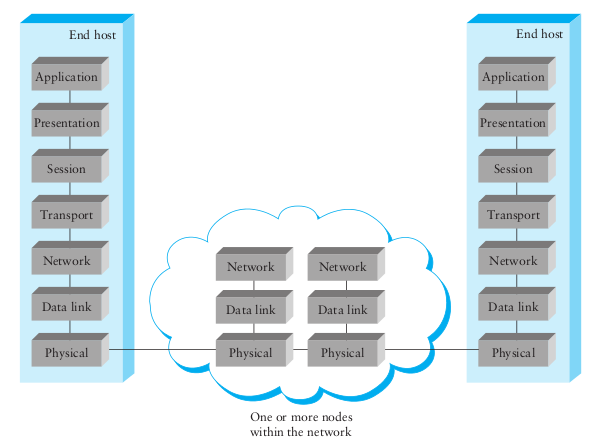
\includegraphics[width=\textwidth/2]{imgs/osi.png}
\end{center}

\subsection{Paquetes IP}

Los paquetes IP\footnote{RFC 791 (IP): https://tools.ietf.org/html/rfc791} son el método principal de intercambio de mensajes entre nodos a nivel de red. Es decir, cuando los nodos pertenecen a distintas redes locales y no tienen acceso la dirección física del otro. El protocolo IP es \textit{best-effort}, por lo tanto existe la posibilidad de que un mensaje nunca llegue a destino. Es más, los routers que implementan RED\footnote{RFC 2309 (RED): https://tools.ietf.org/html/rfc2309}, están configurados para descartar paquetes periódicamente con alguna probabilidad, incluso antes de entrar en un estado de congestión.

\subsection{Paquetes ICMP}

Los paquetes ICMP\footnote{RFC 792 (ICMP): https://tools.ietf.org/html/rfc792} son paquetes de control que no contienen datos, utilizados por los routers para reportar errores en el intercambio de mensajes de una conexión.

\subsection{Traceroute}

Traceroute es una herramienta que permite mostrar la ruta de una conexión entre dos nodos, identificando todos los nodos intermedios y sus respectivos tiempos de demora.
